\chapter{Implementation}
\label{chap:impl}
This chapter gives the detailed description of the implementation of the analyzers of EO intermediate representation. Section \ref{impl:data_structures} desribes the common data structures used by the analyzers. Sections \ref{impl:mutualrec} and \ref{impl:unjustified} describe the analysis algorithms and their implementations.

\section{Data Structures}
\label{impl:data_structures}

\subsection{EO Syntax Tree}
This is a data structure that is used to model the syntactic structure of EO which is used as a starting point for the extraction of more high-level concepts, such as class-objects, method-objects and method calls. It describes EO following the syntax specification from the paper by Bugayenko \cite{eolang}, with slight deviations to account for the specifics of the underlying refined $\varphi$-calculus described in \cite{kudasov}. 

In order to create the parser from the EO code to EO syntax tree we used \textbf{cats-parse} \footnote{\url{https://github.com/typelevel/cats-parse}}, a monadic parser combinator \cite{hill_combinators_1996}  library for Scala.

EO syntax tree is an immutable polymorphic data structure defined \textit{à la carte} \cite{alacarte} \pic{fig:ast}. 
Since the tree is immutable, it can only be altered by constructing the new version, where the old parts of the tree are replaced with new ones. The transformations that construct these new versions of the data structure are known as \textit{optics} \cite{optics}. We used the \textit{monocle} \footnote{\url{https://www.optics.dev/Monocle/}} library for Scala to simplify the generation of the optics that modify the EO syntax tree.  

\begin{figure}
    \lstinputlisting[language=Scala]{code/ast.scala}
    \caption{EO syntax tree definitions (abridged).}
    \label{fig:ast}
\end{figure}
\subsection{Object Tree}
Object Tree is a data strcuture that captures the relationships between objects in an EO program. It is a refinenement of the EO syntax tree, which contains the elements of an EO program relevant to subsequent analysis steps: class-objects, method-objects, extension clauses and method calls. 

EO object tree is also a recursively-defined polymorphic data structure \pic{fig:objtree}. The type parameter $A$ represents the information that is stored for each object in the tree. This information is stored in \textit{info} field of the tree. The field called \textit{nestedObjs} is stores the information about all the nested class-objects. Nested objects are the class-objects that are defined as the attributes of other class objects, just like nested classes in Java. The information about one of the nested objects can be accessed by the key which is of type \textit{Name}. This name identifies the object uniquely because the object can not contain two attributes with the same name.  

\begin{figure}
    \begin{lstlisting}
        final case class ObjectTree[A](
          info: A,
          nestedObjs: Map[Name, ObjectTree[A]]
        ) 
    \end{lstlisting}
    \caption{Object tree}
    \label{fig:objtree}
\end{figure}

\subsection{ObjectInfo}

The first and the most generally-applicable type we use in place of type parameter $A$  is \textit{ObjectInfo} \pic{fig:objinfo}. This type also has two type parameters. The first one, $P$, is responsible for holding the information about the decorated object (or simply parent). The first traversal can only gather the name of the decorated object. 

The second type parameter, $M$, is the type used to store the information about each of the methods. The information captured during the first traversal of EO syntax tree \pic{fig:methodinfo} can be summarised as follows:
\begin{itemize}
    \item \textit{selfArgName} - the name of the free attribute of the method object that is used to capture the calling object. 
    \item \textit{body} - the EO syntax tree node that hold the body of the method. 
    \item \textit{depth} - how deeply the method object is nested in an EO program. For toplevel objects this attribute is $0$. For method objects (that are always defined in the class-objects), this attribute is equal to the depth of the class-object plus one.  
    \item \textit{calls} - a sequence of method calls in the method definition. The \textit{Call} type stores all the necessary information to identify and traverse all the call within the method body:
    \begin{itemize}
        \item depth - depth of the object where the call is located. This value is equal to the depth of the method-object + the relative depth of the method-local object containing the call.
        \item \textit{methodName} - a simple name of the method-object where the call is located.
        \item \textit{callSite} - an optic \cite{optics} which extracts the location of the method-local object where the call is located. 
        \item \textit{callLocation} - an optic \cite{optics} that extracts the location of the EO syntax tree node that defines the method call. 
        \item \textit{args} - the EO syntax tree nodes, which correspond to the arguments of the call, including the \textbf{self} argument.  
    \end{itemize}  
\end{itemize}

\begin{figure}
    \begin{lstlisting}[language=Scala]
      final case class ObjectInfo[P, M](
        name: Name,
        fqn: FQName,
        depth: Int,
        parentInfo: Option[P],
        methods: Map[Name, M],
      )
    \end{lstlisting}
    \caption{ObjectInfo}
    \label{fig:objinfo}
\end{figure}

\begin{figure}
    \begin{lstlisting}[language=Scala]
      final case class MethodInfo(
          selfArgName: String,
          calls: Vector[Call],
          body: EOObj[EOExprOnly],
          depth: Int,
      )
          
      final case class Call(
        depth: BigInt,
        methodName: String,
        callSite: PathToCallSite,
        callLocation: PathToCall,
        args: NonEmptyVector[EOBnd[EOExprOnly]]
      )
    \end{lstlisting}
    \caption{MethodInfo and Call}
    \label{fig:methodinfo}
\end{figure}

\subsection{Partial object tree}
The \textit{ObjectInfo}, where $P$ is the name of the parent object and $M$ is \textit{MethodInfo} can be called the \textit{partial object tree}:
\begin{lstlisting}
    type PartialObjectTree = ObjectTree[
        ObjectInfo[ParentName, MethodInfo]
    ]

\end{lstlisting}

\subsection{Complete object tree}
\label{impl:complete_object_tree}
The so-called \textit{complete object tree} is defined as the following type alias:
\begin{lstlisting}[language=Scala]
  type CompleteObjectTree =
    ObjectTree[
      ObjectInfo[
        LinkToParent,
        MethodInfo
      ]
    ]
\end{lstlisting}
The only thing that distinguishes it from the \textit{partial object tree} is that the parent name is replaced with the special \textit{LinkToParent} type. This type is also an optic \cite{optics} and is essentially a function of the type:
\begin{lstlisting}[language=Scala]
    val linkToParent: 
      CompleteObjectTree => CompleteObjectTree
\end{lstlisting}
It takes the whole object tree of the program and returns the object which represents the decorated object of the object where the link is located.



\section{Detecting Unanticipated Mutual Recursion}
\label{impl:mutualrec}

\subsection{Proposed solution}
\label{impl:mutualrec_algo}
The solution to the problem lies in detecting the cycles in the call-graphs of all the objects. For each class-object in the program, do the following:
\begin{enumerate}
    \item Detect the decorated class-object, all methods, and for each method in the class detect all the methods it calls. If the method that is called exists in the class-object, mark it as \textit{resolved}. Otherwise, mark it as \textit{partially-resolved}. The set of mappings between the methods of the class and the methods that each of the methods calls is considered a \textit{partial call-graph} of the object.
    \item After that the tree is traversed again to convert all the partially-resolved calls to fully resolved calls. To do that we need to calculate the \textit{complete call-graph} of the object, which contains the methods from the object itself, as well as the methods from the decorated object. This is done by \textit{extending} the partial call-graph of the decorated object with the partial call-graph of the decorating objects. Hereinafter we use the terms \textbf{child} and \textbf{parent} to refer to the decorating object and the decorated object respectively. The extension procedure is defined as follows:
          \begin{enumerate}
              \item if the method is present in the parent call-graph, but is absent in the child call-graph, it is left as is.
              \item if the method is present in the child call-graph but does not exist in the parent call-graph, it is added to the parent call-graph.
              \item if the method is present both in the child call-graph and the parent call-graph, all the occurrences of the method in the parent call-graph are replaced by the child's version of the method.
          \end{enumerate}
    \item After the object's call-graph is resolved, perform the depth-first search \cite{dfs} to find the cycles in the complete call-graph. After all the cycles are found, exclude the cycles that contain only the methods from the same object.
\end{enumerate}

\subsection{Implementation}
The first step of the algorithm in \ref{impl:mutualrec_algo} is covered by converting the EO code into a \textit{complete object tree} (section \ref{impl:complete_object_tree}). Then the object tree is converted into a variation of the object tree where all the calls are resolved. This variation is called \textit{ObjectTreeWithResolvedCallgraphs} \pic{fig:mutualrec_program}. For each object, only its fully resolved call-graph is stored. The final step traverses the tree and collects all the cycles in a list of special objects of type \textit{CallChain}. This object represents the sequence of fully-qualified method names that when called would never terminate. Finally, each of such call chains are presented to the user in the form of human-readable strings. 

\begin{figure}
    \begin{lstlisting}[language=Scala]
        type ResolvedCallGraph = 
          Map[Methodname, Set[MethodName]]
        type ObjectTreeWithResolvedCallgraphs =
          ObjectTree[ResolvedCallGraph]
    \end{lstlisting}
    \caption{\textit{ObjectTreeWithResolvedCallgraphs}.}
    \label{fig:mutualrec_program}
\end{figure}

\section{Detecting Unjustified Assumption in Subclass}
\label{impl:unjustified}

\subsection{Proposed Solution}
\label{impl:unjustified_algo}
We propose the following approach for detecting the methods where inlining of the calls may lead to breaking changes in subclasses:
\begin{enumerate}
    \item An \textit{initial} representation of the program is produced. This representation is a tree-like data structure which preserves the nesting relations between objects. So, the objects which contain other objects are the roots of their respective subtrees, whereas the container objects are the subtrees or leaves.
    \item We produce a \textit{revision} of the initial program representation where all the calls to the methods are inlined.
    \item In both versions, for each of the class-objects, for each method in the class-object, a set of \textit{properties} is inferred.  These properties can be thought of as an implicit contract \cite{meyer} of each method. In addition to the implicit properties, the explicit properties which come in the form of \textit{assert} statements in the source code are also taken into account. In order to infer the properties of the method, partial interpretation of its body is performed. The interpretation is limited to basic numeric operations, numeric and boolean values and method calls. The inference rules are described in greater detail in fig. \ref{fig:props}.
    \item After all the properties are inferred, the following predicate should hold true for both the initial and the revised versions:
          \begin{align}
              P_{init} \implies P_{rev}
              \label{fig:implication}
          \end{align}
          If it doesn't hold for some class-object, it means that the revision of one of its superclasses introduces a breaking change, which weakens the precondition of some its methods.
\end{enumerate}

\begin{figure}
  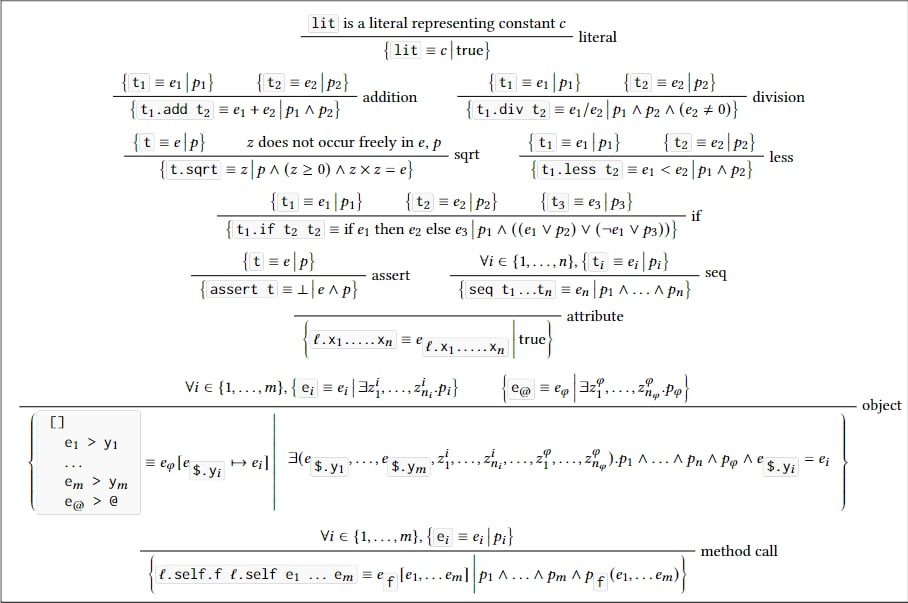
\includegraphics[width=\textwidth]{figs/properties}
  \caption{Rules for property inference in detection of unjustified assumption in subclass.}
  \label{fig:property_inference}
\end{figure}



\subsection{Implementation}
Similarly to the algorithm for the detection of mutual recursion, the tree-like representation of the initial revision of the EO program is done by converting its source code to the \textit{complete object tree} (section \ref{impl:complete_object_tree}). However, in order to produce the revision of the initial program, we needed to implement the inlining procedure for EO syntax tree. This procedure can be summarised as follows:
\begin{enumerate}
  \item Detect all the method calls. This is already done during the construction of the complete object tree.
  \item Replace each method call in the method body with the value of its $\varphi$-attribute (@ symbol in eo).
  \item if the method-object that is inlined contains attributes other than $\varphi$, then:
  \begin{enumerate}
    \item collect these attributes into a separate object called \textit{local\_attrs}. If the attribute with such a name already exists in the object where the call is inlined, resolve the collision by adding a suffix to the newly created object. 
    \item Add this object as a local attribute to the method-object where the call is located. 
    \item Rewire the references to the local attributes inside the $\varphi$ attribute of the methods that is being inlined to their respective attributes in the \textit{local\_attrs} object.
  \end{enumerate}

  \item After the revision of the initial EO code is obtained, the initial object tree and the revised object tree are zipped together in a separate instance of the object tree \pic{fig:zipwithinlined}.

  \item Now that we have all the necessary information about both the initial and revised versions, we need to derive their properties \pic{fig:property_inference}. These properties are encoded as SMTLIB2 \cite{smtlib} programs. We use the \textbf{scala-smtlib} \footnote{\url{https://github.com/regb/scala-smtlib}} library to programmatically construct SMTLIB2-compliant programs. These programs are stored in an auxiliary data structure \ref{fig:property_structure}. This structure has the following fields.
  \item When this structure is constructed for both the initial and revised versions, an implication statement corresponding to the formula \pic{fig:implication} is constructed and passed to the SMT-solver backend. The backend we use in this thesis is called Princess \cite{princess}.
  \item If the solver finds the given to be satisfiable, then there is no error and the revision is considered safe. Otherwise, the revision is considered unsafe and is reported to the user. 
\end{enumerate}

\begin{figure}
\begin{lstlisting}[language=Scala]
  final case class Info(
    forall: List[SortedVar],
    exists: List[SortedVar],
    value: Term,
    properties: Term
  )
\end{lstlisting}
\caption{A data structure for storing the derived properties.}
\label{fig:property_structure}
\end{figure}

\begin{figure}
\begin{lstlisting}[language=Scala]
  final case class MethodInfoForAnalysis(
    selfArgName: String,
    body: EOObj[EOExprOnly],
    depth: Int
  )

  final case class ObjectInfoForAnalysis[P, M](
    methods: Map[EONamedBnd, M],
    parentInfo: Option[P],
    name: Name,
    indirectMethods: Map[
      Name, 
      MethodInfoForAnalysis
    ],
    allMethods: Map[
      Name, 
      MethodInfoForAnalysis
    ]
  )

  type AnalysisInfo = ObjectInfoForAnalysis[
    LinkToParent,
    MethodInfo
  ]
  type InitialAndRevised = ObjectTree[
      (AnalysisInfo, AnalysisInfo)
    ]
\end{lstlisting}
\caption{The object tree used in unjustufied assumption analysis that holds the revised version of the object together with the initial version.}
\label{fig:zipwithinlined}
\end{figure}
